\documentclass[12pt,german]{article}
\usepackage[latin1]{inputenc}
\usepackage{textcomp}
\usepackage{epsf}
\usepackage{german}
\usepackage{float}
\usepackage{hyperref}
\hypersetup{
    colorlinks=true,
    linkcolor=blue,
    filecolor=magenta,      
    urlcolor=cyan,
}
\usepackage{amsmath,amsfonts,amssymb,amsxtra}  % z.B. f�r \text im math-modus
\usepackage{pstricks,pst-node,pst-text,pst-3d}
\usepackage{graphicx}
\pagestyle{empty}
\usepackage{tikz}
\evensidemargin0cm
\oddsidemargin0cm
\textwidth16cm
\textheight24cm
\topmargin-2cm
\parindent 0pt
\newtheorem{aufgabe}{Aufgabe}

\begin{document}
\begin{flushright} Becker \end{flushright}
\vspace{-5mm}
\rule{\linewidth}{0.6mm}
\begin{center}{ \Large Datenstrukturen und Effiziente Algorithmen}\\
{\large Wintersemester 2019}\vspace{-3mm}
\end{center}
\rule{\linewidth}{0.6mm}
\begin{flushleft}
{\bf \large Pr�senzaufgaben 1}
\end{flushleft}

\vspace*{3mm}

\bigskip
{\bf Aufgabe 1.} (Wdh Tiefensuche)\\

{\bf A} Gib eine Adjazenzlisten-Repr�sentation des folgenden Graphen $G=(V,E)$ an.
\medskip
\newline
\centerline{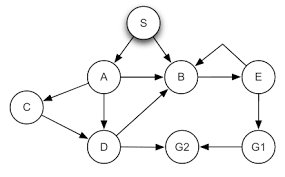
\includegraphics[width=9.8cm]{graph.png}}
\medskip
\newline
{\bf B} Auf Basis dieser Repr�sentation, gib die discover- und finish-times aller Knoten an, startend mit $S$.
\medskip
\newline
{\bf C} Gib eine m�glichst kleine Menge von Kanten $E' \subset E$ an, s.d. $G'=(V,E \setminus E')$ kreisfrei ist. Gib eine topologische Ordnung der Knoten des kreisfreien Graphen an.

\vspace*{8mm}

{\bf Aufgabe 2.} (O-Notation)
\medskip
\newline
{\bf A} Beweise, dass $2n^2 +3n+1 \in O(n^2)$.
\medskip
\newline
{\bf B} Ist $2^{n+1} \in O(2^n)$?
\medskip
\newline
{\bf C} Ist $2^{2n} \in O(2^n)$?
\medskip
\newline


\vspace*{8mm}


{\bf Aufgabe 3.} (Menge der Tiefensuche Kanten ist Wald)\\

Beweise die Aussage aus der Vorlesung:
$(V, E_{pred})$ ist azyklisch.

\newpage


{\bf Aufgabe 4. (Python)} \\

Melde dich auf \href{https://jupyterhub.wolke.uni-greifswald.de}{Jupyter Uni Greifswald} mit deiner Uni-Kennung an.

Kopiere das Notebook \textbf{DFSexperiments.ipynb} von Moodle in dein Verzeichnis und �ffne es.

Wir gehen das Notebook zusammen durch. Dann wollen wir folgendes Problem l�sen:

\medskip 

Finde einen effizienten Algorithmus, der die stark zusammenh�ngenden Komponenten eines gerichteten Graphen ausgibt. 

\medskip 

Ein gerichteter Graph ist stark zusammenh�ngend, wenn zwischen allen geordneten Knotenpaaren ein Pfad existiert. Die stark zusammenh�ngenden Komponenten eines Graphen sind eine Partition der Knoten, sodass jede Teilmenge einen stark zusammenh�ngenden Teilgraphen darstellt und maximal ist.

\medskip 

\textit{Tipp: Benutze DFS (ggf. mehrmals).}

\medskip

{\bf Aufgabe 4. (C++)} \\

Schreibe ein einfaches Programm, das f�r den Graphen aus Aufgabe 1 bei Angabe eines Knotens (zB ./meinProgramm 'A') alle zu diesem Knoten adjazenten Knoten ausgibt.

\textit{Tipp: Benutze den Template Code von �bungsblatt 1.}

\bigskip

\end{document}
